\documentclass[two column]{article}
\usepackage{graphicx}
\usepackage{wrapfig}
\usepackage{tikz}
\usepackage{verbatim}
\usetikzlibrary{shapes}
\usetikzlibrary{math}
\usetikzlibrary{decorations.pathreplacing}

\begin{document}
\title{Modeling the Destruction of the Temple in Judges 16}
\author{Johannes Byle\\Department of Physics\\Wheaton College\\Wheaton, IL}
\maketitle
\section{Abstract}
In this paper we analyze the destruction of the temple in Judges 16 by modeling the temple as a plate resting stacked cylinders. We differentiate between two different ways in which the pillars can move, slipping or tipping, and estimate the force required for each scenario. We also analyze which scenario is more likely given the common materials at the time and estimate the critical angles of the cylinders in the second scenario.
\section{Introduction}
The story of Samson in Judges is one of the most interesting in the entire Bible, his exploits resemble a modern action movie. More interesting than the heroics of the story however is the interesting physics of the destruction of the temple of Judges 16; what would tipping a pillar look like? There are of course several options which are less mechanically interesting, perhaps the pillar simply cracked and broke, or perhaps the pillar fell in one piece. In this paper the assumption is that the pillar did not fail in this way, but rather the pillar made up of several smaller sections stacked on top of each other that can be modeled as stack of rigid cylinders. Although we cannot know for certain that this was the type of pillar that Samson destroyed, pillars made up of stacked did exist in antiquity. This is an interesting physical problem, and there have been several papers published the subject of the stability of stacked items: Hall, John. “Fun with stacking blocks” American Journal of Physics 73 (2005), Ziglar, James. “Analysis of Mechanics in Jenga” Robotics Institute, Carnegie Mellon University.

\begin{figure}
\includegraphics[scale=.75]{Columns.jpg}
\caption{Example of a pillar made of stacked columns in Ephesus, Turkey}
\end{figure}

Ideally I would model the motion of every single block in the pillar from the initial push until it comes to rest. This would make the problem far to complex however, and is far too dependent on the layout of the temple. For example, would the pillars cause the roof to tip and cause the other pillars to fall, or would the roof simply collapse once the pillars fall? I will ignore these questions and instead focus on how much force is required to push the pillars and at what point the pillars will become unstable and fall. 

\section{Theoretical Background}
Aside from modeling the pillar as a stack of cylinders of uniform mass there are several other assumption that need to be made. The first assumption is that the roof will not be significantly affected by the tipping of the pillar. If any of the cylinders in the pillar begin to tip the effective height of the pillar will increase which could cause the force of the roof on the pillar to increase because it is no longer supported by other pillars. I will ignore this in my calculations and assume that the roof simply provides a constant force on the pillar. The third assumption is that there will be two distinct ways the pillar can fall. The first is the low friction regime in which none of the pillars will tip each other due to friction. The second is the high friction regime in which the pillar will not slip but will instead tip both pillars.\footnote{Although not an official physics paper, this resource was incredibly helpful for me in how to distinguish between slipping and tipping. adaptivemap.ma.psu.edu/websites/friction/slipping\_vs\_tipping/ slippingvstipping.html}
In the low friction regime the equations are very simple. The equation for friction is simply the the friction coefficient multiplied by the normal force between the blocks.
$$F_{Friction}=\mu N$$
The torque between the blocks is:
$$\tau=rN$$
Where $r$ is the overhang between the blocks, and $N$ is the normal force between the blocks. The equation for $N$, the force between blocks is:
$$N=mg$$
Where $m$ is the total mass above the blocks and $g$ is the acceleration due to gravity. Thus in the first regime the pillar will become unstable when the block is pushed a distance of $\frac{1}{1+m_{c_1}/F_{roof}}$. The force required to push the block in this regime is $F=\mu(2m_{c_1}+2F_{roof}+m_{c_2})$.

The equations for motion for the high friction regime are slightly different. There are no direct normal forces, there are only torques. The equations for these torques are:
$$\tau_{\perp}=mg\cos\theta$$
$$\tau_{\parallel}=\mu mg\sin\theta$$
Where $m$ is the total mass above the block, $g$ is the acceleration due to gravity, and $\theta$ is the angle between the block and the ground. Parallel and perpendicular are also measured relative to the ground.
The only other equations we will need are the equations for estimating force. We can estimate the force required in the first regime using simply the equation for the force of friction. For the second regime however I will estimate the force required using the work required to lift the roof a the distance required for the blocks to become unstable.

We can use these equations to determine when our system will become unstable. For the first regime it will become unstable once $\tau=rN$ is greater than the force of the roof. For the second regime it will become unstable once the blocks go past their tipping points. The equation for determining when this will occur is:\footnote{demonstrations.wolfram.com/TippingPointOfACylinder/ This source actually had the wrong equation, but it provided me with a useful starting point}
$$\theta=\arctan(r/2h)$$
This equation is not affected by the weight of the roof, as the weight of the roof is constant and acts in the same direction. This means that the critical angle of the cylinders will remain the same.

Based on these equations we can get an estimate for the amount of force required to topple the pillars. The two sources that will take energy in the second regime are the rotation of the blocks and the increase in height of the roof. The two equations of energy that will be useful to us then are the equation for rotational kinetic energy and the equation for gravitational potential energy:
$$E_{rotational}=\frac{1}{2}I\omega^2$$
$$E_{gravitational}=mgh$$
Since the cylinder will be rotating around an edge the moment of inertia will be $I=\frac{1}{4}mr^2+\frac{1}{3}mL^2$ where L is the height of the block. In this case $h$ is not the height of the block but rather the displacement of the roof in the vertical direction. The equation for the total displacement is rather simple and can be described using the Pythagorean theorem and the angles of the blocks. $h=r(\sin\theta_1+\sin\theta_2)$. Since force is proportional to work:
$$W=\int Fds$$
We can calculate the total force using the change in energy.

\section{Methods}
Using the equations detailed in the previous section we get the following diagrams for the forces. The low friction regime is a much simpler diagram as all the forces are perpendicular or parallel to the ground.\\

\begin{figure}[h]
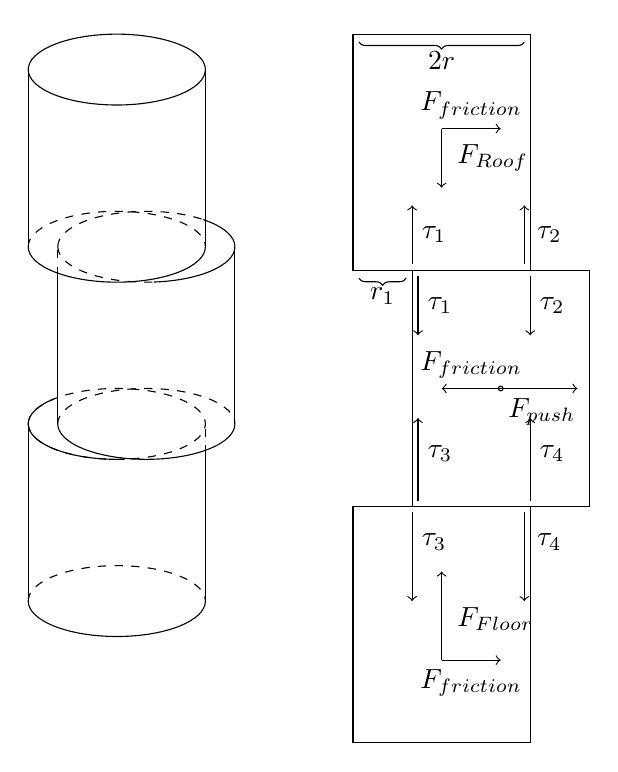
\begin{tikzpicture}[scale = 1.5]
	    
    \tikzmath{\x1 = -1.5;};
    \tikzmath{\x2 = 0;};
    \tikzmath{\x3 = .25;};
    \draw (.75,\x2) arc (0:360:.75 and 0.3);
	\draw (-.75,\x2) -- (-.75,\x1);
	\draw (-.75,\x1) arc (180:360:.75 and 0.3);
	\draw [dashed] (-.75,\x1) arc (180:360:.75 and -0.3);
	\draw (.75,\x1) -- (.75,\x2);

	\tikzmath{\x1 = -3;};
    \tikzmath{\x2 = -1.5;};
    \tikzmath{\x3 = .35;};
	\draw (-.5,\x2-.24) -- (-.5,\x1);
	\draw [dashed] (-.5,\x2-.24) -- (-.5,\x2);
	\draw (-.5,\x1) arc (180:360:.75 and 0.3);
	\draw [dashed] (-.5,\x1) arc (180:360:.75 and -0.3);
	\draw [dashed] (-.5,\x2) arc (180:275:.75 and 0.3);
	\draw [dashed] (-.5,\x2) arc (180:310:.75 and -0.3);
	\draw (1,\x2) arc (360:310:.75 and -0.3);
	\draw (1,\x2) arc (360:275:.75 and 0.3);
	\draw (1,\x1) -- (1,\x2);
	
	\draw (-.75,\x1) arc (180:275:.75 and 0.3);
	\draw (-.75,\x1) arc (180:225:.75 and -0.3);	
	\draw [dashed] (-.75,\x1) arc (180:360:.75 and 0.3);
	\draw [dashed] (-.75,\x1) arc (180:360:.75 and -0.3);	
	
	\tikzmath{\x1 = -4.5;};
    \tikzmath{\x2 = -3;};
    \tikzmath{\x3 = .45;};
	\draw (-.75,\x2) -- (-.75,\x1);
	\draw (-.75,\x1) arc (180:360:.75 and 0.3);
	\draw [dashed] (-.75,\x1) arc (180:360:.75 and -0.3);
	\draw (.75,\x1) -- (.75,\x2-.25);
	\draw [dashed] (.75,\x2-.25) -- (.75,\x2);
 
	\tikzmath{\x1 = .25;};	
	\draw (2,0.3) rectangle (3.5,-1.7);
	\draw (\x1+2.25,-1.7) rectangle (\x1+3.75,-3.7);
	\draw (2,-3.7) rectangle (3.5,-5.7);
	

	
	\draw [->] (\x1+2.3,-3.65) -- (\x1+2.3,-2.95);
	\draw[decoration={brace,mirror,raise=5pt},decorate] (2.05,-1.65) -- node[below=5pt] {$r_1$} (2.45,-1.65);
	\draw[decoration={brace,mirror,raise=5pt},decorate] (2.05,.35) -- node[below=5pt] {$2r$} (3.45,.35);

	\draw [->] (3.5,-3.65) -- (3.5,-2.95);
	\draw [->] (\x1+2.3,-1.75) -- (\x1+2.3,-2.25);
	\node [right] at (\x1+2.3,-2){$\tau_{1}$};
	\node [right] at (\x1+3.25,-2){$\tau_{2}$};
	\node [right] at (\x1+2.3,-3.25){$\tau_{3}$};
	\node [right] at (\x1+3.25,-3.25){$\tau_{4}$};
	\draw [->] (3.5,-1.75) -- (3.5,-2.25);
	\draw [->] (\x1+3,-2.7) -- (\x1+2.5,-2.7);
	\node [above] at (\x1+2.75,-2.7){$F_{friction}$};
	\draw [->] (\x1+3,-2.7) -- (\x1+3.65,-2.7);
	\node [below] at (\x1+3.35,-2.7){$F_{push}$};
	\draw (\x1+3,-2.7) circle (0.02);
	
	\draw [->] (\x1+2.25,-1.65) -- (\x1+2.25,-1.15);
	\draw [->] (3.45,-1.65) -- (3.45,-1.15);
	\draw [->] (2.75,-.5) -- (2.75,-1);
	\node [right] at (2.8,-.75){$F_{Roof}$};	
	\node [right] at (\x1+2.25,-1.4){$\tau_{1}$};
	\node [right] at (3.475,-1.4){$\tau_{2}$};
	\draw [->] (2.75,-.5) -- (3.25,-.5);
	\node [above] at (3,-.5){$F_{friction}$};
	
	\draw [->] (\x1+2.25,-3.75) -- (\x1+2.25,-4.5);
	\draw [->] (3.45,-3.75) -- (3.45,-4.5);
	\node [right] at (\x1+2.25,-4){$\tau_{3}$};
	\node [right] at (3.475,-4){$\tau_{4}$};
	\draw [->] (2.75,-5) -- (2.75,-4.25);
	\node [right] at (2.8,-4.65){$F_{Floor}$};
	\draw [->] (2.75,-5) -- (3.25,-5);
	\node [below] at (3,-5){$F_{friction}$};
	
\end{tikzpicture}
\caption{Model of a section of a pushed pillar in the low friction regime}
\end{figure}

In this case the forces on the blocks can be described with the following equations:\\
$C_2,$ $F_{Friction}=\mu_{C_1C_2}(m_{C_1}+m_{Roof})g+\dots$\\
$\mu_{C_2C_3}(m_{C_1}+m_{C_2}+m_{Roof})g$\\
$C_2,$ $F_{push}=Constant$\\
$C_2,$ $\tau_{1}(r_1-r^2)=\tau_2(r_1+r)$\\
$C_2,$ $F_{C_2 on C_3}=(m_{C_2}+m_{C_1}+m_{Roof})g$\\

$C_1,$ $F_{Friction}=\mu_{C_1C_2}(m_{C_1}+m_{Roof})g$\\
$C_1,$ $F_{Roof}=m_{Roof}g$\\
$C_1,$ $\tau_{1}(r_1-r^2)=\tau_2(r_1+r)$\\
$C_2,$ $\tau_{3}(r_1-r^2)=\tau_4(r_1+r)$\\
$C_1,$ $F_{C_2onC_1}=(m_{C_1}+m_{Roof})g$\\

$C_3,$ $F_{Friction}=\mu_{C_2C_3}(m_{C_1}+m_{C_2}+m_{Roof})g$\\
$C_3,$ $\tau_{3}(r_1-r^2)=\tau_4(r_1+r)$\\
$C_3,$ $F_{C_3}=(m_{C_1}+m_{C_2}+m_{C_3}+m_{Roof})g$\\

The high-friction regime is more complicated as the torques act in different directions.

\begin{figure}[h]

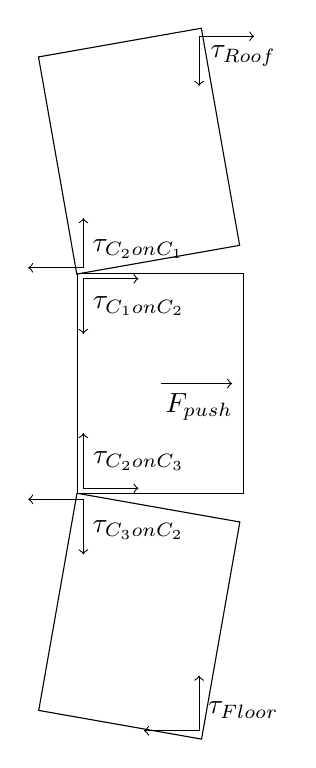
\begin{tikzpicture}[scale = 1.4] 
	
	\draw [rotate=10] (1.91,-0.07) rectangle (3.41,-2.07);
	\draw (2.25,-1.7) rectangle (3.75,-3.7);
	\draw [rotate=-10](2.85,-3.25) rectangle (4.35,-5.25);
	
	%\node[right] at (4,-.5) {$C_1,$ $\tau_{Roof}=m_{Roof}g\cos\theta$};
	%\node[right] at (4,-.75) {$C_1,$ $\tau_{Friction}=\mu_{Roof}m_{Roof}\sin\theta$};
	
	\draw [->] (3,-2.7) -- (3.65,-2.7);
	\node [below] at (3.35,-2.7){$F_{push}$};

	

	\draw [->] (2.3,-1.75) -- (2.3,-2.25);
	\draw [->] (2.3,-1.75) -- (2.8,-1.75);
	\node [right] at (2.3,-2){$\tau_{C_1 on C_2}$};
	
	\draw [->] (2.3,-3.65) -- (2.8,-3.65);
	\draw [->] (2.3,-3.65) -- (2.3,-3.15);
	\node [right] at (2.3,-3.4){$\tau_{C_2 on C_3}$};

	\draw [->] (2.3,-1.65) -- (2.3,-1.2);
	\draw [->] (2.3,-1.65) -- (1.8,-1.65);
	\node [above] at (2.8,-1.65){$\tau_{C_2 on C_1}$};
	\draw [->] (3.35,.45) -- (3.35,0);
	\draw [->] (3.35,.45) -- (3.85,.45);
	\node [below] at (3.75,.45){$\tau_{Roof}$};
	
	\draw [->] (2.3,-3.75) -- (2.3,-4.25);
	\draw [->] (2.3,-3.75) -- (1.8,-3.75);
	\node [above] at (2.8,-4.2){$\tau_{C_3 on C_2}$};
	
	\draw [->] (3.35,-5.85) -- (3.35,-5.35);
	\draw [->] (3.35,-5.85) -- (2.85,-5.85);
	\node [below] at (3.75,-5.5){$\tau_{Floor}$};
	


\end{tikzpicture}
\caption{Model of a section of a pushed pillar in the high friction regime}
\end{figure}

In this case the forces on the blocks can be described with the following equations:\\
$C_1,$ $\tau_{Roof}=m_{Roof}g\cos\theta$\\
$C_1,$ $\tau_{Friction}=\mu_{Roof}m_{Roof}\sin\theta$\\
$C_2,$ $\tau_{C_1onC_2}=(m_{c_1}+m_{Roof})g\cos\theta$\\
$C_2,$ $\tau_{Friction}=\mu_{Roof}(m_{c_1}+m_{Roof})\sin\theta$\\
$C_3,$ $\tau_{C_2onC_3}=(m_{c_1}+m_{c_2}+m_{Roof})g\cos\theta$\\
$C_3,$ $\tau_{Friction}=\mu_{Roof}(m_{c_1}+m_{c_2}+m_{Roof})\sin\theta$\\

Using these equations I was able to create graphs of the force required to push the pillars, as well as the critical angle. Since the density of granite or marble is a known constant the only truly unknown variables are the mass of the roof and the radius of the pillars. We can narrow down minimum values for the roof size using the fact that there were $3,000$ Philistines in the temple. Since crowds generally don't exceed a density of $6$ people per meter squared the roof must have cross sectional area of at least $3000/6$ or $500 m^2$.\footnote{``Dynamics of crowd disasters: An empirical study" Dirk Helbing, Anders Johansson, and Habib Zein Al-Abideen Phys. Rev. E 75, 046109 Published 18 April 2007} To get starting values for $r$ and $h$ I used statistics from the temple depicted in figure 1, which according to Pliny had pillars $18m$ high with a radius of $0.6m$.

Using these starting variables I was able to visualize the possible critical angles and forces. I initially used two while loops to create a matrix of all possible values for $r$ and $m_{roof}$. I visualized these matrices using the surf() function. One of these saddle functions roughly resembled a paraboliod, and thus properly creating a graph from this function was somewhat difficult. I ended up converting the surf function to a more easily readable line graph in order to display the graph in a more easily understandable way. Another difficulty I had was that one of the equations I had was incorrect (my equation for the tipping point). But I did not notice this until I saw the data.

\section{Results}
The following graphs all have a few key shared assumptions. The value for the density of material is $2500kg/m^3$ for all cases. Furthermore, the height and number of pillars is constant as well at $18m$ and $5$ sections.

The low friction regime is the simplest in terms of force. The force required to push the blocks to their tipping point is essentially linear since although the mass of the pillars increases with the square of the radius the mass of the blocks is small compared to mass of the roof. 

\begin{figure}[h]
\includegraphics[scale=.4]{341_3.jpg}
\caption{The force required to push the columns in the low friction regime}
\end{figure}

The high friction regime is much more interesting as the critical angle is important and thus the radius has a much more important effect on the final force required.

This data still has a lot of uncertainty since we do not know the exact design of the temple. This data shows that there is a variability of $14\times10^6N$. In comparison the space shuttle main engine produces only $1.8\times10^6N$ of thrust, thus the variability is quite large. And that does not even account for all the other variables such as density of rock or height of pillars. We can narrow down this uncertainty somewhat by looking at which regime is more likely. Whether or not we need to model using the high friction or low friction models depends on whether the block will tip or slip. The equation for determining whether or not a block will tip or slip is $M_{push/f}=M_{g/N}$. \footnote{adaptivemap.ma.psu.edu/websites/friction} In the case of stacked columns we can see that we will have to compare the friction force with the force required to tip the block $\mu F_g$ vs $\frac{F_{g}r}{h}$. Since marble and granite have a coefficient of friction close to .5 this suggests that unless the height of the pillars is very small they will most likely tip.

\begin{figure}[h]
\includegraphics[scale=.4]{341_1.jpg}
\caption{The critical angle of the columns in the high friction regime}
\end{figure}

\begin{figure}[h]
\includegraphics[scale=.4]{341_2.jpg}
\caption{The force required to push the columns in the high friction regime}
\end{figure}

\section{Conclusion}
Whether or not the pillars of that Samson toppled resembled stacked cylinders is a question that will remain impossible to answer, however if the temple did indeed resemble a flat rigid block sitting on top of stacked rigid cylinder the temples destruction would be an awesome sight to behold. Even if the pillars did not follow our models exactly, tipping the pillars would require forces somewhere close or within where the data predicts. Thus, even with a low estimate Samson would have had to use forces comparable to the thrust of the space shuttle main engines. Although we could use these models to create a 3-D depiction of the temple and analyze how the location of the pillars affects the collapse, or exactly what the buckling would look like this analysis answers the most important and obvious questions of force and critical angle.

\end{document}
